\documentclass[amsmath,amssymb,superscriptaddress]{revtex4-1}

\usepackage{graphicx}% Include figure files
\usepackage{dcolumn}% Align table columns on decimal point
\usepackage{bm}% bold math
\usepackage[detect-all]{siunitx}
\usepackage{hyperref}% add hypertext capabilities
\usepackage{xr}
\usepackage{mhchem}
\renewcommand{\thefigure}{S\arabic{figure}}
\renewcommand{\theequation}{S\arabic{equation}}
\renewcommand{\thesection}{S\arabic{section}}
\renewcommand{\thetable}{S\Roman{table}}

\graphicspath{{./figures/}}

\begin{document}                  % DO NOT DELETE THIS LINE

\title{SI for ``Assessing coarse-grained simulation for the analysis of lipid monolayer reflectometry''}

\author{A.~R. McCluskey}
\email{a.r.mccluskey@bath.ac.uk}
\affiliation{Department of Chemistry, University of Bath, Claverton Down,
Bath, BA2 7AY, UK}
\affiliation{Diamond Light Source, Harwell Campus, Didcot, OX11 0DE, UK}

\author{J. Grant}
\affiliation{Computing Services, University of Bath, Claverton Down, Bath, BA2 7AY, UK}

\author{A. J. Smith}
\affiliation{Diamond Light Source, Harwell Campus, Didcot, OX11 0DE, UK}

\author{J. L. Rawle}
\affiliation{Diamond Light Source, Harwell Campus, Didcot, OX11 0DE, UK}

\author{D. J. Barlow}
\affiliation{Institute of Pharmaceutical Science, King's College London, London, SE1 9NH, UK}

\author{M. J. Lawrence}
\affiliation{Division of Pharmacy and Optometry, University of Manchester, Manchester, M13 9PT, UK}

\author{S.~C. Parker}
\affiliation{Department of Chemistry, University of Bath, Claverton Down,
Bath, BA2 7AY, UK}

\author{K.~J. Edler}
\email{k.edler@bath.ac.uk}
\affiliation{Department of Chemistry, University of Bath, Claverton Down,
Bath, BA2 7AY, UK}

\date{\today}

\maketitle                        % DO NOT DELETE THIS LINE

This Supplementary Information document is only part of a fully reproducible analysis workflow. The complete workflow, along with all datasets, figure files, and analysis/plotting scripts is available at \url{https://github.com/arm61/sim_vs_trad} (DOI: 10.5281/zenodo.2587486) under a CC BY-SA 4.0 license.


\section{Abel\`{e}s matrix formalism}

The Abel\`{e}s matrix formalism method invoked the use of the chemically-consistent monolayer model.
For this it is necessary to have the scattering length of the individual head and tail components of the different lipid contrasts, these are given in Table \ref{tab:scat}.
%
\begin{table}[h]
\small
  \caption{\ The different scattering lengths of the head and tail lipid components. }
  \label{tab:scat}
  \begin{tabular*}{0.48\textwidth}{@{\extracolsep{\fill}}lllll}
    \hline
    Contrast & d$_{13}$-DSPC & d$_{70}$-DSPC & d$_{83}$-DSPC & h-DSPC  \\
    \hline
    $b_{\text{head}}$\SI{10e-4}{\angstrom} & 19.54 & 11.21 & 24.75 & 6.01 \\
    $b_{\text{tail}}$\SI{10e-4}{\angstrom} & -3.58 & 69.32 & 69.32 & -3.58 \\
    \hline
  \end{tabular*}
\end{table}
%

In order to apply the Abel\`{e}s matrix formalism, the SLD for the layers, $N$, were determined as detailed in the text of the paper.
This $\text{SLD}_N$ allows for the determination of the wavevector, $k_N$ at a particular $q$-vector in the $N$-th layer, by considering the difference in SLD between the layer $N$ and the semi-infinite layer 0 (Figure 1),
%
\begin{equation}
    k_N^2 = k_0^2 - 4\pi(\text{SLD}_N - \text{SLD}_0)
\end{equation}
%
where $k_0 = q/2$ and $\text{SLD}_0$ is the SLD of the superphase.
For each of the interfaces between two layers, it is possible to evaluate a Fresnel coefficient, $r_{N,N+1}$, which describes the refraction of the probing radiation occurring between the layers $N$ and $N+1$,
%
\begin{equation}
    r_{N,N+1} = \frac{k_N - k_{N+1}}{k_N + k_{N+1}}\exp{(-2k_Nk_{N+1}\sigma^2_{N, N+1})}.
\end{equation}
%
The exponential factor is due to the fact that the layer is unlikely to be perfectly smooth and will therefore have some roughness, this is modelled as an error function with some width $\sigma_{N,N+1}$ \cite{nevot_caracterisation_1980}.
A phase factor, $\beta_N$, which considers the layer thickness, $d_N$, and the wavevector can then be found,
%
\begin{equation}
    \beta_N =
    \begin{cases}
        0 + 0i & N = 0, \\
        k_N d_N & N > 0.
    \end{cases}
\end{equation}
%
These two parameters are then brought together in the characteristic matrix for the layer, $C_N$,
%
\begin{equation}
    C_N =
    \begin{bmatrix}
        \exp{\beta_N} & r_{N,N+1} \exp{\beta_N} \\
        r_{N,N+1}\exp{-\beta_N} & \exp{-\beta_N}
    \end{bmatrix},
\end{equation}
%
the product sum of which gives a resultant matrix for each value of $q$,
%
\begin{equation}
    M(q) = \prod_{n=0}^{n_{\text{max}}} C_N.
\end{equation}
%
From this matrix, the reflected intensity, $R(q)$, can be determined,
%
\begin{equation}
    R(q) = \frac{|M(q)_{21}|}{|M(q)_{11}|}.
\end{equation}
%

\section{MARTINI potential model considerations}
It was noted in the work of Koutsioubas \cite{koutsioubas_combined_2016}, that the use of the MARTINI water bead, could result in the ordering of the water structure.
This can be observed in the scattering length density profile (Figure \ref{fig:mart}) when the layer thickness of \SI{1}{\angstrom} was used.
In an effort to reduce this effect, a larger layer thickness, or \SI{4}{\angstrom} was used for the MARTINI potential model.
%
\begin{figure*}
 \centering
 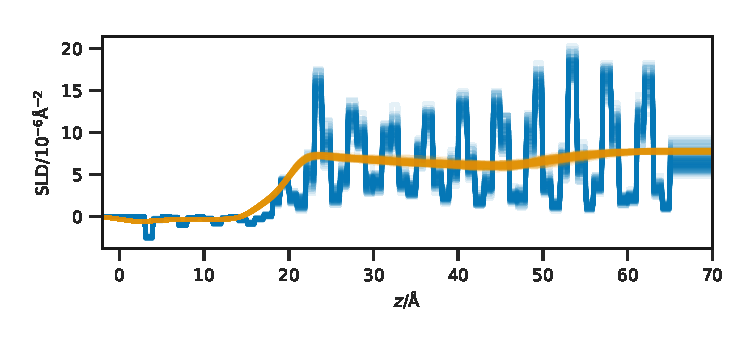
\includegraphics[width=0.49\textwidth]{martini_order}
 \caption{The scattering length density profile from the MARTINI simulation, at an effective surface pressure of \SI{30}{\milli\newton\per\meter} with a layer thickness of \SI{1}{\angstrom} (blue) and \SI{4}{\angstrom} (orange). }
 \label{fig:mart}
\end{figure*}
%

A negative effect of this large layer thickness was that the smoothness associated with the \SI{1}{\angstrom} layer was lost.
In an effort to reproduce this, an interfacial roughness of \SI{0.4}{\angstrom} was included in the model.
We believe that this gave the MARTINI potential model a fair chance to reproduce the experimental data.
However, as is noted in the main text of the paper, the systematic beading problem leads to more severe issues.

\section{Reflectometry profiles}
Figures \ref{fig:sp20} through \ref{fig:sp50} show the reflectometry profiles for each of the analysis methods that correspond to surface pressures of \SI{20}{\milli\newton\per\meter}, \SI{40}{\milli\newton\per\meter}, and \SI{50}{\milli\newton\per\meter}.
The profile that corresponds to a surface pressure of \SI{30}{\milli\newton\per\meter} is given in Figure 4.
Tables~\ref{tab:chi20} through \ref{tab:chi50} give the $\chi^2$ for each contrast, average $\chi^2$, and standard deviation for each method at each surface pressure not covered in the main paper.

%
\begin{figure*}
 \centering
 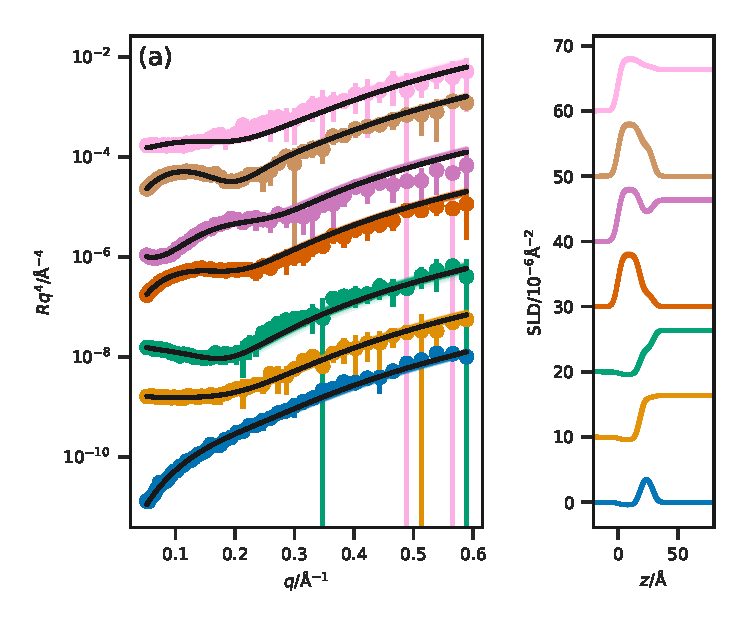
\includegraphics[width=0.49\textwidth]{dspc_20_ref_sld}
 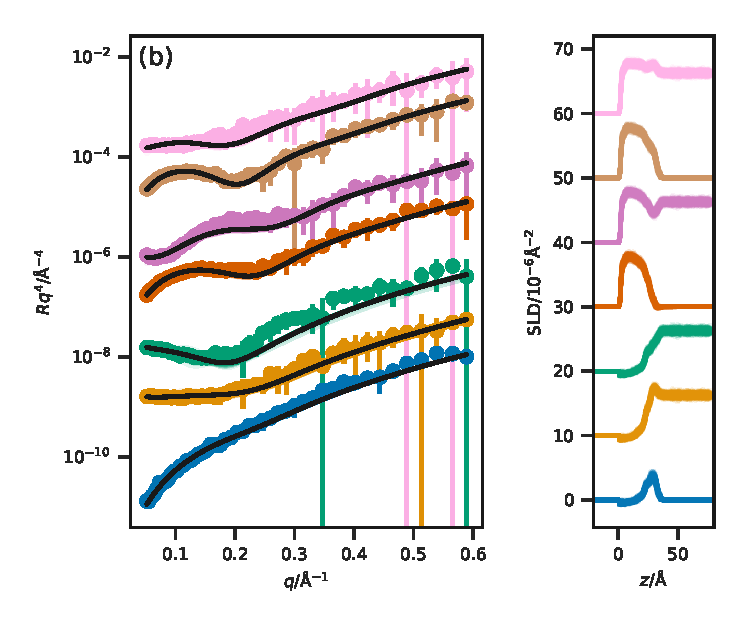
\includegraphics[width=0.49\textwidth]{dspc_slipids_20_ref_sld} \\
 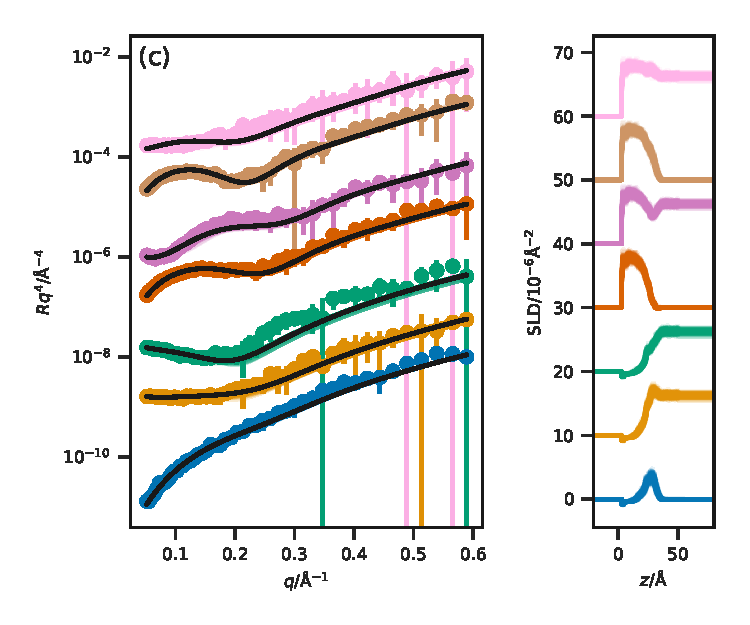
\includegraphics[width=0.49\textwidth]{dspc_berger_20_ref_sld}
 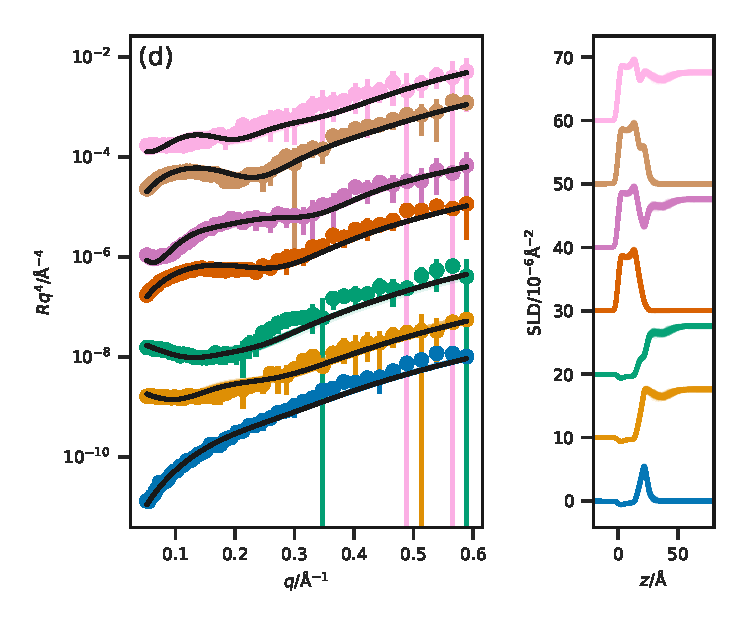
\includegraphics[width=0.49\textwidth]{dspc_martini_20_ref_sld}
 \caption{A comparison of the reflectometry and SLD profiles obtained from (a) the monolayer model, (b) the Slipid simulation, (c) the Berger force-force simulation, and (d) the MARTINI potential model simulation at a surface pressure of \SI{20}{\milli\newton\per\meter}. From top-to-bottom the contrasts are as follows; \ce{d_{83}}-\ce{D2O}, \ce{d_{83}}-ACMW, \ce{d_{70}}-\ce{D2O}, \ce{d_{70}}-ACMW, h-\ce{D2O}, \ce{d_{13}}-\ce{D2O}, \ce{d_{13}}-ACMW. The different contrast reflectometry profiles have been offset in the \emph{y}-axis by an order of magnitude and the SLD profiles offset in the \emph{y}-axis by \SI{1e-6}{\per\square\angstrom}, for clarity.}
 \label{fig:sp20}
\end{figure*}
%
%
\begin{figure*}
 \centering
 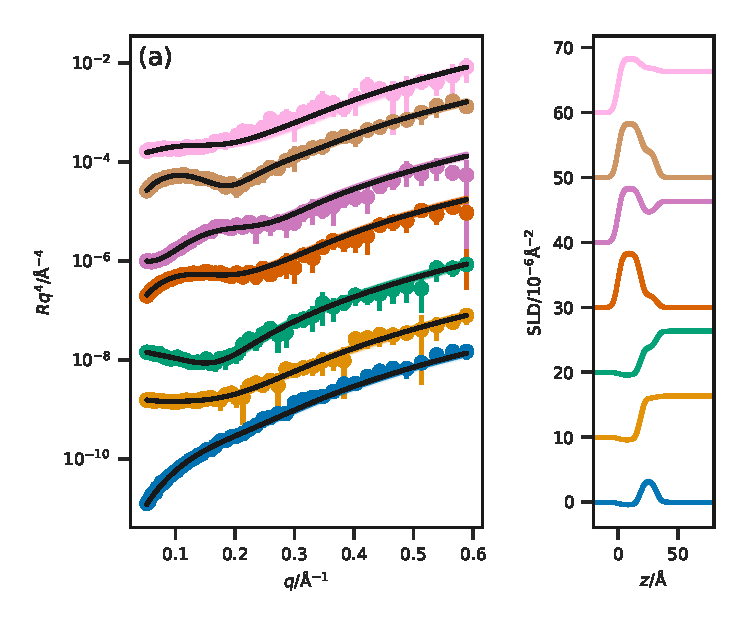
\includegraphics[width=0.49\textwidth]{dspc_40_ref_sld}
 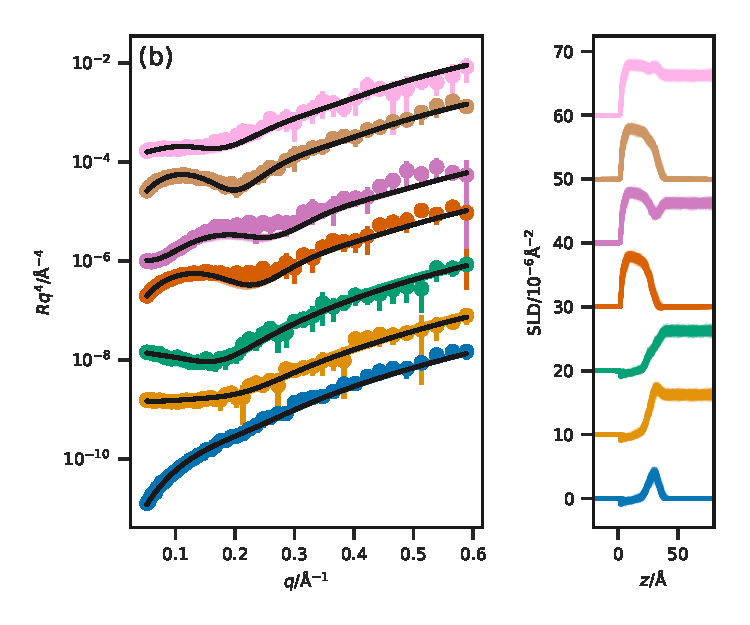
\includegraphics[width=0.49\textwidth]{dspc_slipids_40_ref_sld} \\
 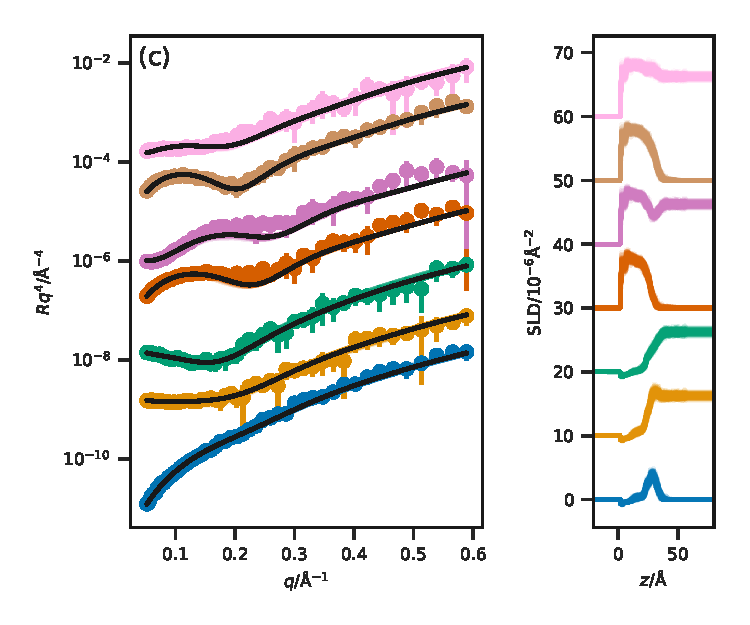
\includegraphics[width=0.49\textwidth]{dspc_berger_40_ref_sld}
 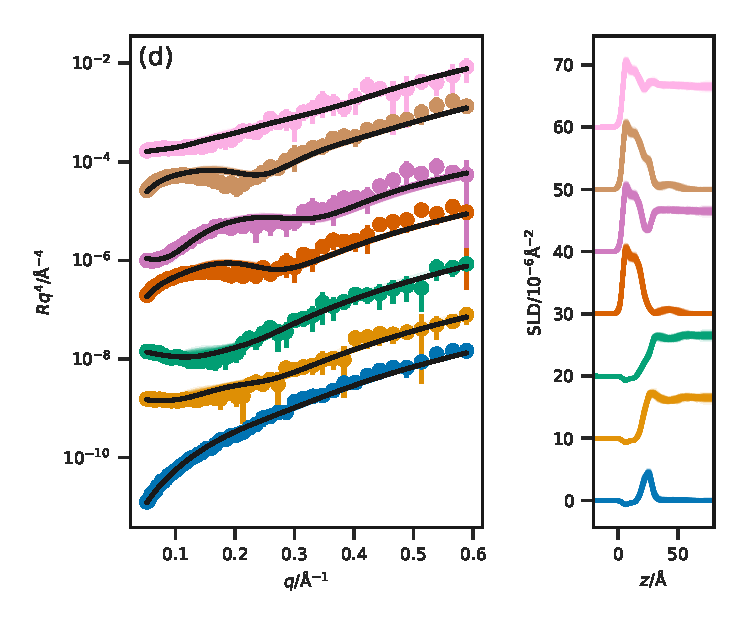
\includegraphics[width=0.49\textwidth]{dspc_martini_40_ref_sld}
 \caption{A comparison of the reflectometry and SLD profiles obtained from (a) the monolayer model, (b) the Slipid simulation, (c) the Berger force-force simulation, and (d) the MARTINI potential model simulation at a surface pressure of \SI{40}{\milli\newton\per\meter}. From top-to-bottom the contrasts are as follows; \ce{d_{83}}-\ce{D2O}, \ce{d_{83}}-ACMW, \ce{d_{70}}-\ce{D2O}, \ce{d_{70}}-ACMW, h-\ce{D2O}, \ce{d_{13}}-\ce{D2O}, \ce{d_{13}}-ACMW. The different contrast reflectometry profiles have been offset in the \emph{y}-axis by an order of magnitude and the SLD profiles offset in the \emph{y}-axis by \SI{1e-6}{\per\square\angstrom}, for clarity.}
 \label{fig:sp40}
\end{figure*}
%
%
\begin{figure*}
 \centering
 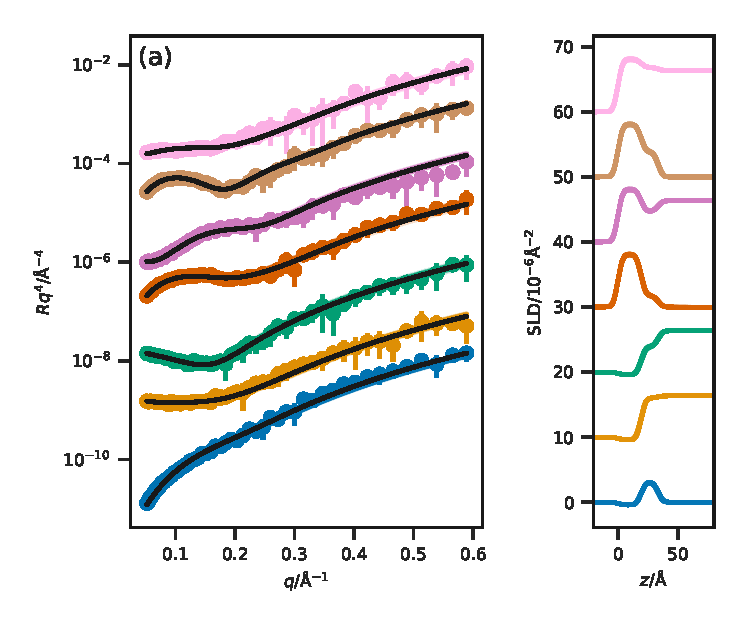
\includegraphics[width=0.49\textwidth]{dspc_50_ref_sld}
 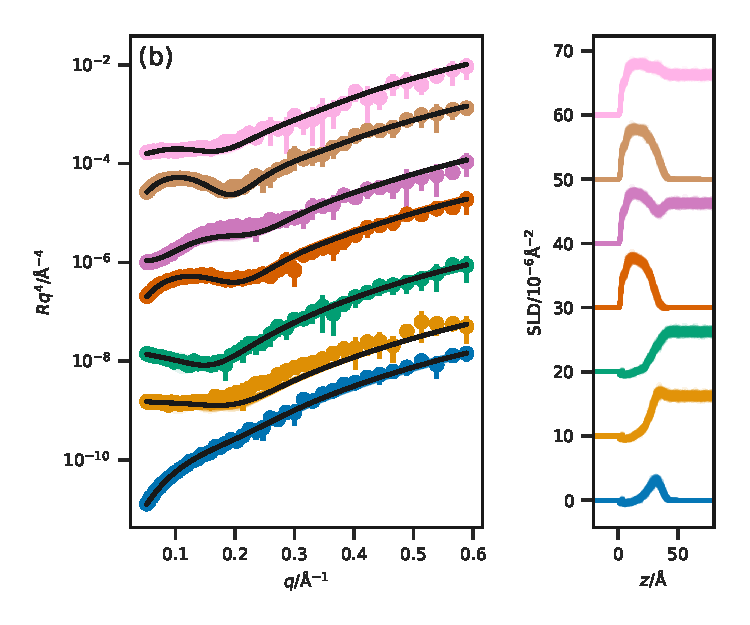
\includegraphics[width=0.49\textwidth]{dspc_slipids_50_ref_sld} \\
 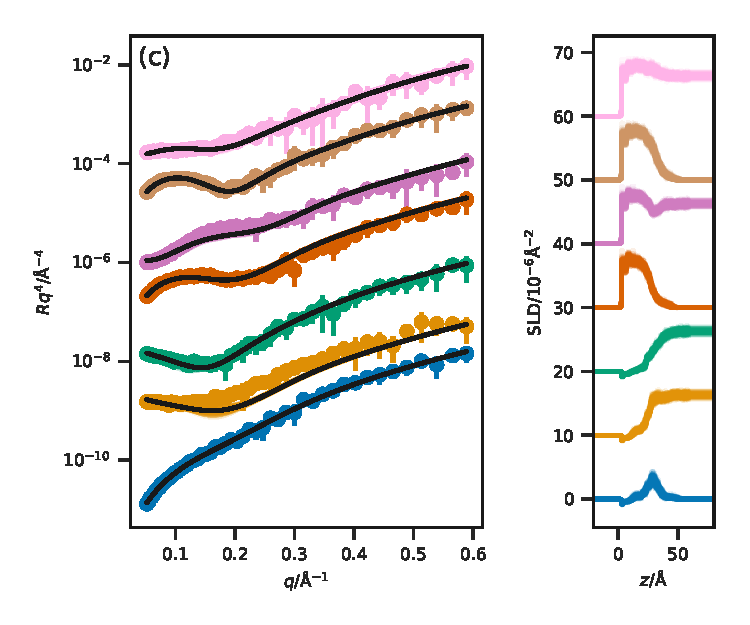
\includegraphics[width=0.49\textwidth]{dspc_berger_50_ref_sld}
 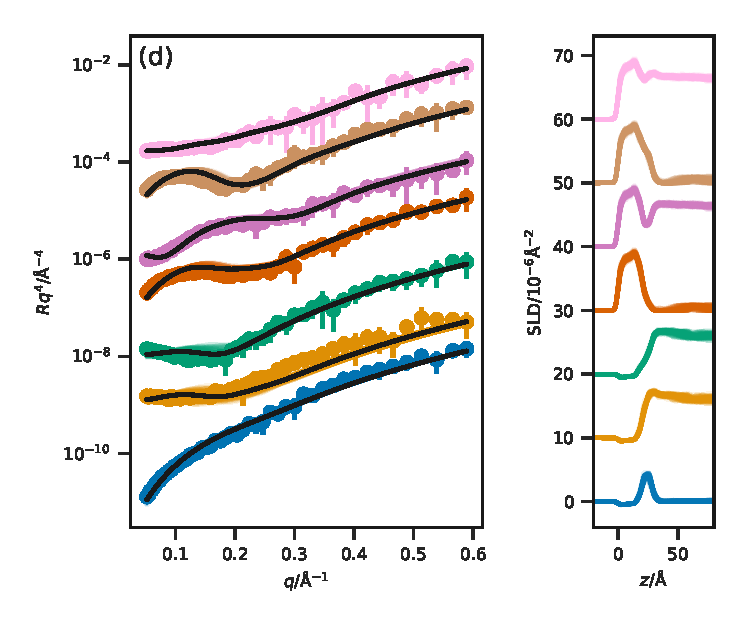
\includegraphics[width=0.49\textwidth]{dspc_martini_50_ref_sld}
 \caption{A comparison of the reflectometry and SLD profiles obtained from (a) the monolayer model, (b) the Slipid simulation, (c) the Berger force-force simulation, and (d) the MARTINI potential model simulation at a surface pressure of \SI{50}{\milli\newton\per\meter}. From top-to-bottom the contrasts are as follows; \ce{d_{83}}-\ce{D2O}, \ce{d_{83}}-ACMW, \ce{d_{70}}-\ce{D2O}, \ce{d_{70}}-ACMW, h-\ce{D2O}, \ce{d_{13}}-\ce{D2O}, \ce{d_{13}}-ACMW. The different contrast reflectometry profiles have been offset in the \emph{y}-axis by an order of magnitude and the SLD profiles offset in the \emph{y}-axis by \SI{1e-6}{\per\square\angstrom}, for clarity.}
 \label{fig:sp50}
\end{figure*}
%
%
\begin{table*}
\small
  \caption{\ The goodness-of-fit between the calculated and experimental
  reflectometry profile at a surface pressure of
  \SI{20}{\milli\newton\per\metre}.}
  \label{tab:chi20}
  \begin{tabular*}{\textwidth}{@{\extracolsep{\fill}}lllll}
    \hline
    Contrast & Monolayer model & Slipid & Berger & MARTINI \\
    \hline
    h-\ce{D2O} & \input{../output/traditional/dspc_20_20_hd2o_chi.txt} &
    \input{../output/simulation/dspc_slipids_20_hd2o_chi.txt} &
    \input{../output/simulation/dspc_berger_20_hd2o_chi.txt} &
    \input{../output/simulation/dspc_martini_20_hd2o_chi.txt} \\
    \ce{d_{13}}-ACMW & \input{../output/traditional/dspc_20_20_d13acmw_chi.txt} &
    \input{../output/simulation/dspc_slipids_20_d13acmw_chi.txt} &
    \input{../output/simulation/dspc_berger_20_d13acmw_chi.txt} &
    \input{../output/simulation/dspc_martini_20_d13acmw_chi.txt} \\
    \ce{d_{13}}-\ce{D2O} & \input{../output/traditional/dspc_20_20_d13d2o_chi.txt} &
    \input{../output/simulation/dspc_slipids_20_d13d2o_chi.txt} &
    \input{../output/simulation/dspc_berger_20_d13d2o_chi.txt} &
    \input{../output/simulation/dspc_martini_20_d13d2o_chi.txt} \\
    \ce{d_{70}}-ACMW & \input{../output/traditional/dspc_20_20_d70acmw_chi.txt} &
    \input{../output/simulation/dspc_slipids_20_d70acmw_chi.txt} &
    \input{../output/simulation/dspc_berger_20_d70acmw_chi.txt} &
    \input{../output/simulation/dspc_martini_20_d70acmw_chi.txt} \\
    \ce{d_{70}}-\ce{D2O} & \input{../output/traditional/dspc_20_20_d70d2o_chi.txt} &
    \input{../output/simulation/dspc_slipids_20_d70d2o_chi.txt} &
    \input{../output/simulation/dspc_berger_20_d70d2o_chi.txt} &
    \input{../output/simulation/dspc_martini_20_d70d2o_chi.txt} \\
    \ce{d_{83}}-ACMW & \input{../output/traditional/dspc_20_20_d83acmw_chi.txt} &
    \input{../output/simulation/dspc_slipids_20_d83acmw_chi.txt} &
    \input{../output/simulation/dspc_berger_20_d83acmw_chi.txt} &
    \input{../output/simulation/dspc_martini_20_d83acmw_chi.txt} \\
    \ce{d_{83}}-\ce{D2O} & \input{../output/traditional/dspc_20_20_d83d2o_chi.txt} &
    \input{../output/simulation/dspc_slipids_20_d83d2o_chi.txt} &
    \input{../output/simulation/dspc_berger_20_d83d2o_chi.txt} &
    \input{../output/simulation/dspc_martini_20_d83d2o_chi.txt} \\
    \hline
    Average$\pm$Standard deviation &
    \input{../output/traditional/dspc_20_20_all_chi.txt} &
    \input{../output/simulation/dspc_slipids_20_all_chi.txt} &
    \input{../output/simulation/dspc_berger_20_all_chi.txt} &
    \input{../output/simulation/dspc_martini_20_all_chi.txt} \\
    \hline
  \end{tabular*}
\end{table*}
%
%
\begin{table*}
\small
  \caption{\ The goodness-of-fit between the calculated and experimental
  reflectometry profile at a surface pressure of
  \SI{40}{\milli\newton\per\metre}.}
  \label{tab:chi40}
  \begin{tabular*}{\textwidth}{@{\extracolsep{\fill}}lllll}
    \hline
    Contrast & Monolayer model & Slipid & Berger & MARTINI \\
    \hline
    h-\ce{D2O} & \input{../output/traditional/dspc_40_40_hd2o_chi.txt} &
    \input{../output/simulation/dspc_slipids_40_hd2o_chi.txt} &
    \input{../output/simulation/dspc_berger_40_hd2o_chi.txt} &
    \input{../output/simulation/dspc_martini_40_hd2o_chi.txt} \\
    \ce{d_{13}}-ACMW & \input{../output/traditional/dspc_40_40_d13acmw_chi.txt} &
    \input{../output/simulation/dspc_slipids_40_d13acmw_chi.txt} &
    \input{../output/simulation/dspc_berger_40_d13acmw_chi.txt} &
    \input{../output/simulation/dspc_martini_40_d13acmw_chi.txt} \\
    \ce{d_{13}}-\ce{D2O} & \input{../output/traditional/dspc_40_40_d13d2o_chi.txt} &
    \input{../output/simulation/dspc_slipids_40_d13d2o_chi.txt} &
    \input{../output/simulation/dspc_berger_40_d13d2o_chi.txt} &
    \input{../output/simulation/dspc_martini_40_d13d2o_chi.txt} \\
    \ce{d_{70}}-ACMW & \input{../output/traditional/dspc_40_40_d70acmw_chi.txt} &
    \input{../output/simulation/dspc_slipids_40_d70acmw_chi.txt} &
    \input{../output/simulation/dspc_berger_40_d70acmw_chi.txt} &
    \input{../output/simulation/dspc_martini_40_d70acmw_chi.txt} \\
    \ce{d_{70}}-\ce{D2O} & \input{../output/traditional/dspc_40_40_d70d2o_chi.txt} &
    \input{../output/simulation/dspc_slipids_40_d70d2o_chi.txt} &
    \input{../output/simulation/dspc_berger_40_d70d2o_chi.txt} &
    \input{../output/simulation/dspc_martini_40_d70d2o_chi.txt} \\
    \ce{d_{83}}-ACMW & \input{../output/traditional/dspc_40_40_d83acmw_chi.txt} &
    \input{../output/simulation/dspc_slipids_40_d83acmw_chi.txt} &
    \input{../output/simulation/dspc_berger_40_d83acmw_chi.txt} &
    \input{../output/simulation/dspc_martini_40_d83acmw_chi.txt} \\
    \ce{d_{83}}-\ce{D2O} & \input{../output/traditional/dspc_40_40_d83d2o_chi.txt} &
    \input{../output/simulation/dspc_slipids_40_d83d2o_chi.txt} &
    \input{../output/simulation/dspc_berger_40_d83d2o_chi.txt} &
    \input{../output/simulation/dspc_martini_40_d83d2o_chi.txt} \\
    \hline
    Average$\pm$Standard deviation &
    \input{../output/traditional/dspc_40_40_all_chi.txt} &
    \input{../output/simulation/dspc_slipids_40_all_chi.txt} &
    \input{../output/simulation/dspc_berger_40_all_chi.txt} &
    \input{../output/simulation/dspc_martini_40_all_chi.txt} \\
    \hline
  \end{tabular*}
\end{table*}
%
%
\begin{table*}
\small
  \caption{\ The goodness-of-fit between the calculated and experimental
  reflectometry profile at a surface pressure of
  \SI{50}{\milli\newton\per\metre}.}
  \label{tab:chi50}
  \begin{tabular*}{\textwidth}{@{\extracolsep{\fill}}lllll}
    \hline
    Contrast & Monolayer model & Slipid & Berger & MARTINI \\
    \hline
    h-\ce{D2O} & \input{../output/traditional/dspc_50_50_hd2o_chi.txt} &
    \input{../output/simulation/dspc_slipids_50_hd2o_chi.txt} &
    \input{../output/simulation/dspc_berger_50_hd2o_chi.txt} &
    \input{../output/simulation/dspc_martini_50_hd2o_chi.txt} \\
    \ce{d_{13}}-ACMW & \input{../output/traditional/dspc_50_50_d13acmw_chi.txt} &
    \input{../output/simulation/dspc_slipids_50_d13acmw_chi.txt} &
    \input{../output/simulation/dspc_berger_50_d13acmw_chi.txt} &
    \input{../output/simulation/dspc_martini_50_d13acmw_chi.txt} \\
    \ce{d_{13}}-\ce{D2O} & \input{../output/traditional/dspc_50_50_d13d2o_chi.txt} &
    \input{../output/simulation/dspc_slipids_50_d13d2o_chi.txt} &
    \input{../output/simulation/dspc_berger_50_d13d2o_chi.txt} &
    \input{../output/simulation/dspc_martini_50_d13d2o_chi.txt} \\
    \ce{d_{70}}-ACMW & \input{../output/traditional/dspc_50_50_d70acmw_chi.txt} &
    \input{../output/simulation/dspc_slipids_50_d70acmw_chi.txt} &
    \input{../output/simulation/dspc_berger_50_d70acmw_chi.txt} &
    \input{../output/simulation/dspc_martini_50_d70acmw_chi.txt} \\
    \ce{d_{70}}-\ce{D2O} & \input{../output/traditional/dspc_50_50_d70d2o_chi.txt} &
    \input{../output/simulation/dspc_slipids_50_d70d2o_chi.txt} &
    \input{../output/simulation/dspc_berger_50_d70d2o_chi.txt} &
    \input{../output/simulation/dspc_martini_50_d70d2o_chi.txt} \\
    \ce{d_{83}}-ACMW & \input{../output/traditional/dspc_50_50_d83acmw_chi.txt} &
    \input{../output/simulation/dspc_slipids_50_d83acmw_chi.txt} &
    \input{../output/simulation/dspc_berger_50_d83acmw_chi.txt} &
    \input{../output/simulation/dspc_martini_50_d83acmw_chi.txt} \\
    \ce{d_{83}}-\ce{D2O} & \input{../output/traditional/dspc_50_50_d83d2o_chi.txt} &
    \input{../output/simulation/dspc_slipids_50_d83d2o_chi.txt} &
    \input{../output/simulation/dspc_berger_50_d83d2o_chi.txt} &
    \input{../output/simulation/dspc_martini_50_d83d2o_chi.txt} \\
    \hline
    Average$\pm$Standard deviation &
    \input{../output/traditional/dspc_50_50_all_chi.txt} &
    \input{../output/simulation/dspc_slipids_50_all_chi.txt} &
    \input{../output/simulation/dspc_berger_50_all_chi.txt} &
    \input{../output/simulation/dspc_martini_50_all_chi.txt} \\
    \hline
  \end{tabular*}
\end{table*}
%

\section{Intrisic surface plots}

Figures~\ref{fig:waters20} to \ref{fig:waters50} show the intrinsic density profiles for water at the air-water interface, for each of the surface pressures not covered in the paper; \SIlist{20;40;50}{\milli\newton\per\meter}.
%
\begin{figure}
\centering
  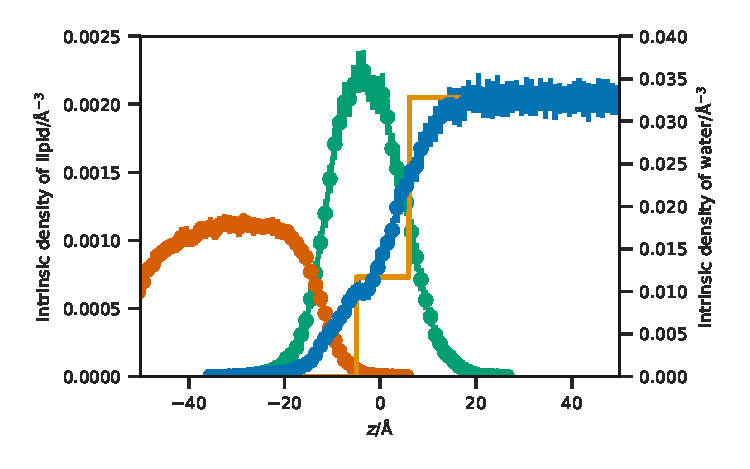
\includegraphics[width=0.48\textwidth]{water_20}
  \caption{The simulation time-averaged intrinsic density profile of the water molecules at the interface, where the phosphorus atoms of the lipid heads create the intrinsic surface at $z=$\SI{0}{\angstrom} (blue dots), at an APM associated with a surface pressure of \SI{20}{\milli\newton\per\meter} and the equivalent scattering length density from the chemically-consistent model (orange line).}
  \label{fig:waters20}
\end{figure}
%
%
\begin{figure}
\centering
  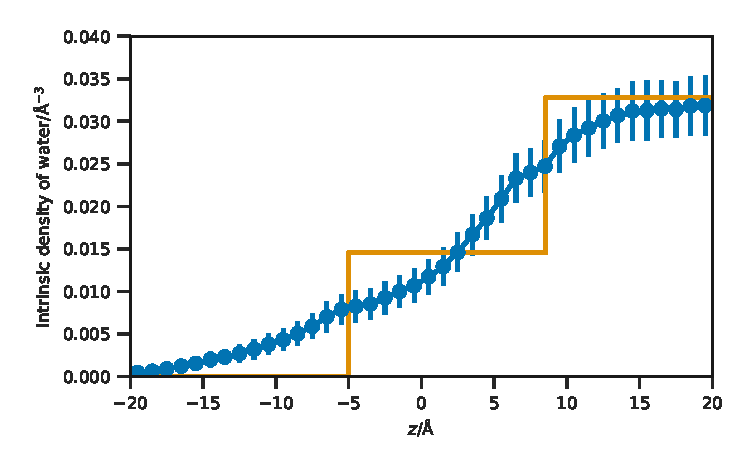
\includegraphics[width=0.48\textwidth]{water_40}
  \caption{The simulation time-averaged intrinsic density profile of the water molecules at the interface, where the phosphorus atoms of the lipid heads create the intrinsic surface at $z=$\SI{0}{\angstrom} (blue dots), at an APM associated with a surface pressure of \SI{40}{\milli\newton\per\meter} and the equivalent scattering length density from the chemically-consistent model (orange line).}
  \label{fig:waters40}
\end{figure}
%
%
\begin{figure}
\centering
  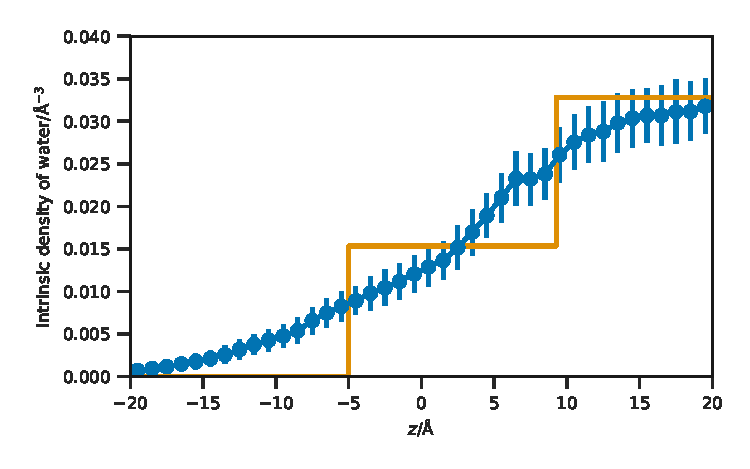
\includegraphics[width=0.48\textwidth]{water_50}
  \caption{The simulation time-averaged intrinsic density profile of the water molecules at the interface, where the phosphorus atoms of the lipid heads create the intrinsic surface at $z=$\SI{0}{\angstrom} (blue dots), at an APM associated with a surface pressure of \SI{50}{\milli\newton\per\meter} and the equivalent scattering length density from the chemically-consistent model (orange line).}
  \label{fig:waters50}
\end{figure}
%

\section{Quantification of roughness}

Tables~\ref{tab:spread1} to \ref{tab:spread3} show the mean, \SI{95}{\percent} quantile and spread for the positions of each part of the lipid for each of the surface pressures not covered in the paper; \SIlist{20;40;50}{\milli\newton\per\meter}.
%
\begin{table}[h]
\small
  \caption{\ The mean, \SI{95}{\percent} quantile, and their spread for the position of atoms representative of difference parts of the lipid, at a surface pressure of \SI{20}{\milli\newton\per\meter}.}
  \label{tab:spread1}
  \begin{tabular*}{0.48\textwidth}{@{\extracolsep{\fill}}llll}
    \hline
    Atom & Mean/\si{\angstrom} & \SI{95}{\percent} quantile/\si{\angstrom} & Spread/\si{\angstrom} \\
    \hline
    Start-Head & \input{../output/simulation/slipids_mean_N_20.txt} & \input{../output/simulation/slipids_uq_N_20.txt} & \input{../output/simulation/slipids_position_N_20.txt} \\
    Mid-Head & \input{../output/simulation/slipids_mean_P_20.txt} & \input{../output/simulation/slipids_uq_P_20.txt} & \input{../output/simulation/slipids_position_P_20.txt} \\
    End-Head & \input{../output/simulation/slipids_mean_C2_20.txt} & \input{../output/simulation/slipids_uq_C2_20.txt} & \input{../output/simulation/slipids_position_C2_20.txt} \\
    \hline
    Start-Tail 1 & \input{../output/simulation/slipids_mean_C21_20.txt} & \input{../output/simulation/slipids_uq_C21_20.txt} & \input{../output/simulation/slipids_position_C21_20.txt} \\
    Start-Tail 2 & \input{../output/simulation/slipids_mean_C31_20.txt} & \input{../output/simulation/slipids_uq_C31_20.txt} & \input{../output/simulation/slipids_position_C31_20.txt} \\
    Mid-Tail 1 & \input{../output/simulation/slipids_mean_C29_20.txt} & \input{../output/simulation/slipids_uq_C29_20.txt} & \input{../output/simulation/slipids_position_C29_20.txt} \\
    Mid-Tail 2 & \input{../output/simulation/slipids_mean_C39_20.txt} & \input{../output/simulation/slipids_uq_C39_20.txt} & \input{../output/simulation/slipids_position_C39_20.txt} \\
    End-Tail 1 & \input{../output/simulation/slipids_mean_8C21_20.txt} & \input{../output/simulation/slipids_uq_8C21_20.txt} & \input{../output/simulation/slipids_position_8C21_20.txt} \\
    End-Tail 2 & \input{../output/simulation/slipids_mean_8C31_20.txt} & \input{../output/simulation/slipids_uq_8C31_20.txt} & \input{../output/simulation/slipids_position_8C31_20.txt} \\
    \hline
  \end{tabular*}
\end{table}
%
%
\begin{table}[h]
\small
  \caption{\ The mean, \SI{95}{\percent} quantile, and their spread for the position of atoms representative of difference parts of the lipid, at a surface pressure of \SI{40}{\milli\newton\per\meter}.}
  \label{tab:spread2}
  \begin{tabular*}{0.48\textwidth}{@{\extracolsep{\fill}}llll}
    \hline
    Atom & Mean/\si{\angstrom} & \SI{95}{\percent} quantile/\si{\angstrom} & Spread/\si{\angstrom} \\
    \hline
    Start-Head & \input{../output/simulation/slipids_mean_N_40.txt} & \input{../output/simulation/slipids_uq_N_40.txt} & \input{../output/simulation/slipids_position_N_40.txt} \\
    Mid-Head & \input{../output/simulation/slipids_mean_P_40.txt} & \input{../output/simulation/slipids_uq_P_40.txt} & \input{../output/simulation/slipids_position_P_40.txt} \\
    End-Head & \input{../output/simulation/slipids_mean_C2_40.txt} & \input{../output/simulation/slipids_uq_C2_40.txt} & \input{../output/simulation/slipids_position_C2_40.txt} \\
    \hline
    Start-Tail 1 & \input{../output/simulation/slipids_mean_C21_40.txt} & \input{../output/simulation/slipids_uq_C21_40.txt} & \input{../output/simulation/slipids_position_C21_40.txt} \\
    Start-Tail 2 & \input{../output/simulation/slipids_mean_C31_40.txt} & \input{../output/simulation/slipids_uq_C31_40.txt} & \input{../output/simulation/slipids_position_C31_40.txt} \\
    Mid-Tail 1 & \input{../output/simulation/slipids_mean_C29_40.txt} & \input{../output/simulation/slipids_uq_C29_40.txt} & \input{../output/simulation/slipids_position_C29_40.txt} \\
    Mid-Tail 2 & \input{../output/simulation/slipids_mean_C39_40.txt} & \input{../output/simulation/slipids_uq_C39_40.txt} & \input{../output/simulation/slipids_position_C39_40.txt} \\
    End-Tail 1 & \input{../output/simulation/slipids_mean_8C21_40.txt} & \input{../output/simulation/slipids_uq_8C21_40.txt} & \input{../output/simulation/slipids_position_8C21_40.txt} \\
    End-Tail 2 & \input{../output/simulation/slipids_mean_8C31_40.txt} & \input{../output/simulation/slipids_uq_8C31_40.txt} & \input{../output/simulation/slipids_position_8C31_40.txt} \\
    \hline
  \end{tabular*}
\end{table}
%
%
\begin{table}[h]
\small
  \caption{\ The mean, \SI{95}{\percent} quantile, and their spread for the position of atoms representative of difference parts of the lipid, at a surface pressure of \SI{50}{\milli\newton\per\meter}.}
  \label{tab:spread3}
  \begin{tabular*}{0.48\textwidth}{@{\extracolsep{\fill}}llll}
    \hline
    Atom & Mean/\si{\angstrom} & \SI{95}{\percent} quantile/\si{\angstrom} & Spread/\si{\angstrom} \\
    \hline
    Start-Head & \input{../output/simulation/slipids_mean_N_50.txt} & \input{../output/simulation/slipids_uq_N_50.txt} & \input{../output/simulation/slipids_position_N_50.txt} \\
    Mid-Head & \input{../output/simulation/slipids_mean_P_50.txt} & \input{../output/simulation/slipids_uq_P_50.txt} & \input{../output/simulation/slipids_position_P_50.txt} \\
    End-Head & \input{../output/simulation/slipids_mean_C2_50.txt} & \input{../output/simulation/slipids_uq_C2_50.txt} & \input{../output/simulation/slipids_position_C2_50.txt} \\
    \hline
    Start-Tail 1 & \input{../output/simulation/slipids_mean_C21_50.txt} & \input{../output/simulation/slipids_uq_C21_50.txt} & \input{../output/simulation/slipids_position_C21_50.txt} \\
    Start-Tail 2 & \input{../output/simulation/slipids_mean_C31_50.txt} & \input{../output/simulation/slipids_uq_C31_50.txt} & \input{../output/simulation/slipids_position_C31_50.txt} \\
    Mid-Tail 1 & \input{../output/simulation/slipids_mean_C29_50.txt} & \input{../output/simulation/slipids_uq_C29_50.txt} & \input{../output/simulation/slipids_position_C29_50.txt} \\
    Mid-Tail 2 & \input{../output/simulation/slipids_mean_C39_50.txt} & \input{../output/simulation/slipids_uq_C39_50.txt} & \input{../output/simulation/slipids_position_C39_50.txt} \\
    End-Tail 1 & \input{../output/simulation/slipids_mean_8C21_50.txt} & \input{../output/simulation/slipids_uq_8C21_50.txt} & \input{../output/simulation/slipids_position_8C21_50.txt} \\
    End-Tail 2 & \input{../output/simulation/slipids_mean_8C31_50.txt} & \input{../output/simulation/slipids_uq_8C31_50.txt} & \input{../output/simulation/slipids_position_8C31_50.txt} \\
    \hline
  \end{tabular*}
\end{table}
%

\bibliography{paper.bib}


\end{document}                    % DO NOT DELETE THIS LINE
